\documentclass[a4paper,12pt]{article}

\title{addFC -- additional tools for FreeCAD}
\author{Golodnikov Sergey}
\date{\today}


\usepackage[left=2cm,right=2cm,top=2cm,bottom=2cm]{geometry}
\usepackage{fontspec}
\setmainfont{PT Astra Serif}
\usepackage[ddmmyyyy]{datetime}
\renewcommand{\dateseparator}{.}
\usepackage{graphicx}
\usepackage{caption}
\usepackage[
	pdfauthor={Golodnikov Sergey},
	pdftitle={Additional tools for FreeCAD},
	pdfsubject={addFC},
	colorlinks=true,
	linkcolor=blue]{hyperref}




\begin{document}
\maketitle




\section{Goals and objectives}

\begin{itemize}
	\item Generate a BOM based on the model.
	\item Batch processing of sheet metal parts.
	\item Assistance in creating design documentation.
	\item Library of elements and nodes.
	\item Process automation.\\
\end{itemize}

The main purpose of the workbench is to simplify the work with large and «complex» assemblies, especially with assemblies containing sheet metal parts. «Complex» I mean parametric models (assemblies) with a large number of objects and nodes in the form of links (App::Link). The main point is to reuse components.

\begin{figure}[htp]
	\centering
	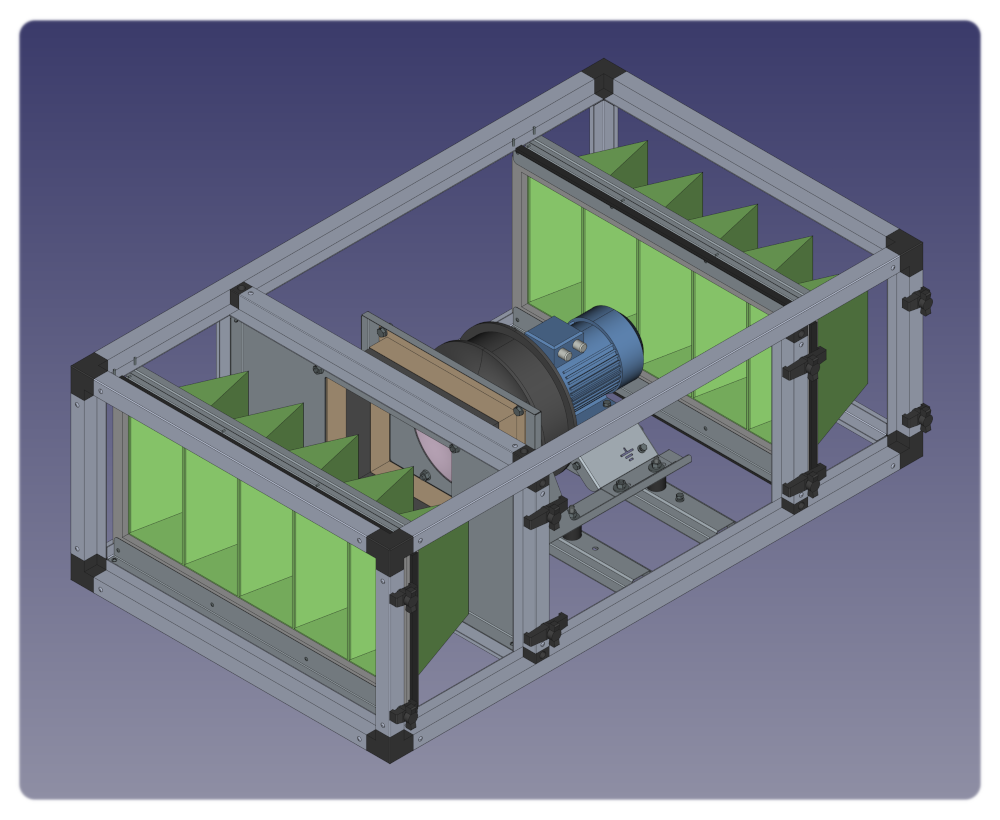
\includegraphics[scale=0.46]{img/assembly_example.png}
	\caption{Example of a «complex» assembly}
	\label{sec:assembly_example}
\end{figure}

\begin{center}\emph{The logic of work is based on adding custom properties to objects, giving them certain semantic meanings.}\end{center}




\section{Toolbar}

When you select the \textbf{addFC workbench}, its toolbar will become available, it looks like this:

\begin{figure}[htp]
	\centering
	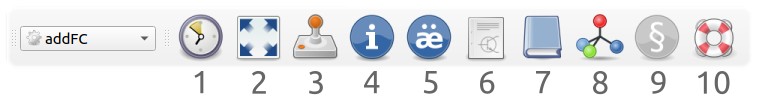
\includegraphics[scale=0.8]{img/toolbar.png}
	\caption{Toolbar}
	\label{sec:toolbar}
\end{figure}

\begin{flushleft}Tools in order:\end{flushleft}
\begin{enumerate}
	\item Open last working file -- \textbf{Recent File} (Alt+Shift+R).\label{sec:1}
	\item Isometry and fit all -- \textbf{Display} (Alt+Shift+D).\label{sec:2}
	\item Managing a parametric model -- \textbf{Model Control} (Alt+Shift+C).\label{sec:3}
	\item Bill of Materials (BOM) -- \textbf{Specification} (Alt+Shift+S).\label{sec:4}
	\item Filling an object with properties -- \textbf{Add Properties} (Alt+Shift+A).\label{sec:5}
	\item Create a drawing based on a template -- \textbf{Creating a Drawing} (Alt+Shift+I).\label{sec:6}
	\item Library of elements and nodes -- \textbf{Library} (Alt+Shift+L).\label{sec:7}
	\item Exploded view -- \textbf{Explode} (Alt+Shift+E).\label{sec:8}
    \item Creating a pipeline using coordinates -- \textbf{Pipe} (Alt+Shift+P).\label{sec:9}
    \item Help -- \textbf{Help and Examples}.\label{sec:10}
\end{enumerate}

Note: FreeCAD allows you to create additional toolbars, I recommend taking advantage of this and creating your own toolbar from the most popular functions to display it on your main workbench, for example in PartDesign.

\pagebreak




\section{Help and examples}

The workbench includes samples that you can study to better understand the principles of its operation, to open one of them, use the \hyperref[sec:10]{Help and Examples} command on the toolbar.
The most suitable example is \textbf{Assembly}, which will be discussed in this guide.

\begin{figure}[htp]
	\centering
	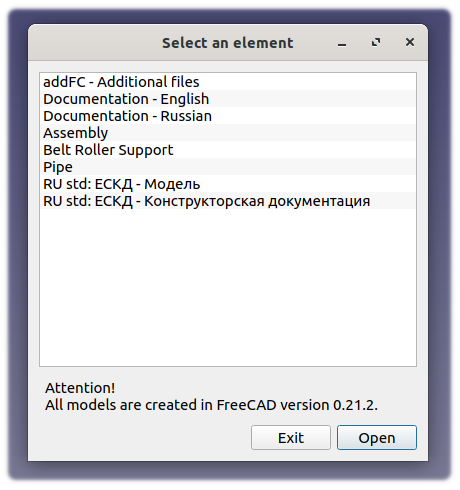
\includegraphics[scale=1]{img/assistant.png}
	\caption{Help and examples}
	\label{sec:assistant}
\end{figure}

\begin{itemize}
	\item \textbf{Additional files} -- supporting files such as templates, fonts.
	\item \textbf{Documentation} -- documentation for using the workbench (this file).
	\item \textbf{Assembly} и \textbf{Belt Roller Support} -- examples of assemblies and working with user properties. Assembly -- parametric assembly.
	\item \textbf{Pipe} -- example of using the tool \hyperref[sec:9]{Pipe}.
	\item \textbf{RU std: ЕСКД} -- example of design according to USDD standards.\\Unified System for Design Documentation -- Russia.
\end{itemize}

\pagebreak




\section{Preferences}

\begin{figure}[htp]
	\centering
	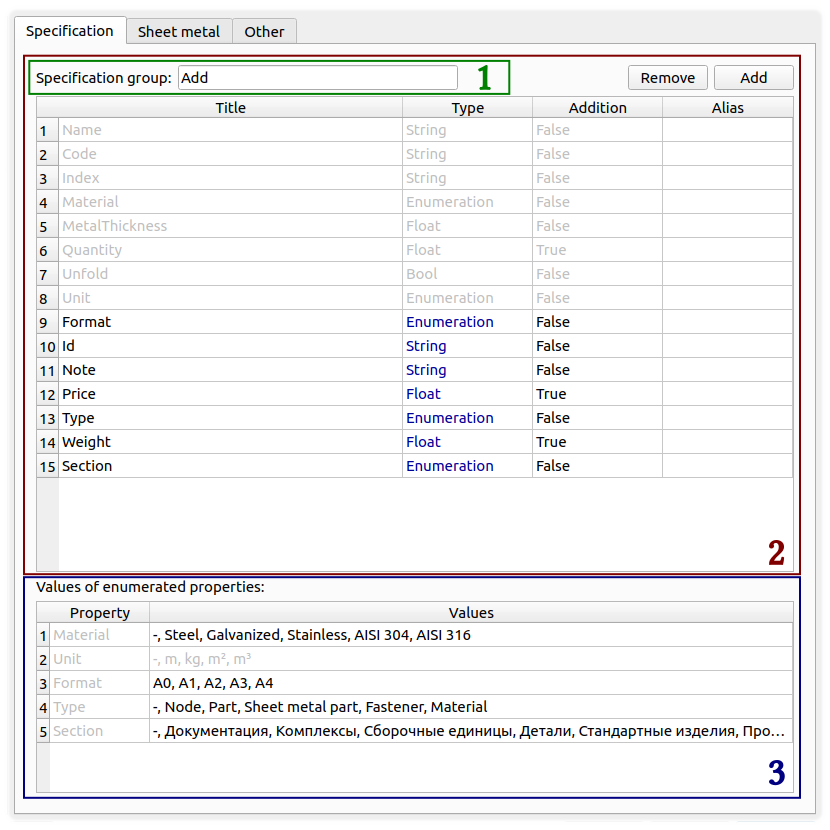
\includegraphics[width=1.0\textwidth]{img/pref_specification.png}
	\caption{Specification (BOM) preferences}
	\label{sec:pref_specification}
\end{figure}

\subsection{Area 1 -- Name for grouping properties}
The properties that we add to objects will be combined into a special group called \textbf{«Add»}. This will facilitate visual perception and will not allow our properties to be mixed with standard ones.

\pagebreak


\subsection{Area 2 -- User properties}

This table contains all the properties available for use.
\begin{itemize}
	\item \textbf{Title} -- property name (important: Latin characters only).
	\item \textbf{Type} -- property value type available for use:
	\begin{itemize}
		\item \textbf{Bool} -- boolean data type (true или false).
		\item \textbf{Enumeration} -- a list of predefined values.
		\item \textbf{Float}.
		\item \textbf{Integer}.
		\item \textbf{String}.
	\end{itemize}
	\item \textbf{Addition} -- indicates the need to sum all property values ​​(example: total assembly mass).
	\item \textbf{Alias} -- a property alias, a value that will replace \textbf{Title} when displaying or exporting a specification (allows you to eliminate the restriction on Latin characters).
\end{itemize}

\begin{flushleft}The \textbf{Remove} and \textbf{Add} buttons, respectively, allow you to delete a property selected in the table or add a row to create a new one.\end{flushleft}

\subsection{Area 3 -- Lists of predefined values}
All properties with the \textbf{Enumeration} data type appear in this area.\\In the \textbf{Values} ​​column -- comma-separated values ​​to form a list.


\subsection{Object properties}

Inactive properties and values ​​in the table are basic and required for the workbench to work correctly.

\begin{center}\emph{Properties should give meaning to FreeCAD objects.}\end{center}

\begin{itemize}
	\item \textbf{Name} -- the name of the object is the most important property, the program works with elements only if they have a name. The name should reflect the essence of the object.
	\item \textbf{Code} -- element designation.
	\item \textbf{Index} -- an identifier for determining the position of an object in an assembly.
	\item \textbf{Material} -- the material of the object (enumeration). This is an important property for sheet metal, when creating a flat part view (unfold) for galvanized and stainless steel, different coefficients are used, and this property is also taken into account when saving the scan to an external file. Additionally, you can link density and cost to this property to automatically calculate the mass and cost of the object.
	\item \textbf{MetalThickness} -- short designation: \textbf{MT}.
	\item \textbf{Node} -- The name of the node to which the object belongs is useful for dividing the final specification into groups. Note: If missing, the document name is used.
	\item \textbf{Price} -- cost price of an object (can be specified by an equation linked to the material).
	\item \textbf{Unfold} -- determines the need to create a flat view (unfold) for a specific object (relevant only for sheet metal parts).
	\item \textbf{Weight} -- object mass.
	\item \textbf{Quantity} and \textbf{Unit} of measurement \textbf{(-, m, kg, m², m³)}. For piece items, the default value in most cases is one, «pcs» \textbf{(-)}. Any combination is available for different materials: for example, a seal length of \textbf{1.2 m} or a quantity of insulation of \textbf{4.2 m²}. Important: values ​​are summed for objects of the same name.
\end{itemize}


\subsection{Additional properties}

These properties are not essential (\emph{they can be removed}), but nevertheless they are useful in work:

\begin{itemize}
	\item \textbf{Format} -- paper format of documentation for a specific object (enumeration).
	\item \textbf{Id} -- some object identifier for communication with another program.
	\item \textbf{Note} -- any note, reminder or clarification.
	\item \textbf{Type} -- object type (enumeration). Useful property for grouping elements when displaying or exporting a BOM.
	\item \textbf{Section} -- specification sections, USDD standard requirement.\\Unified System for Design Documentation -- Russia.
\end{itemize}

\begin{center}\emph{To account for an object by the program, only the \textbf{Name} property is required, all others are used as needed.}\end{center}

\begin{figure}[htp]
	\centering
	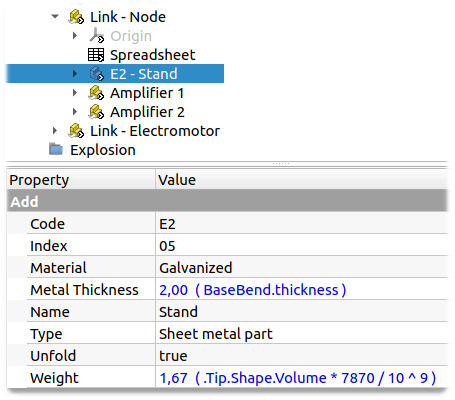
\includegraphics[scale=0.8]{img/properties.png}
	\caption{Example of an object with filled in properties}
	\label{sec:properties}
\end{figure}

\pagebreak

\begin{figure}[htp]
	\centering
	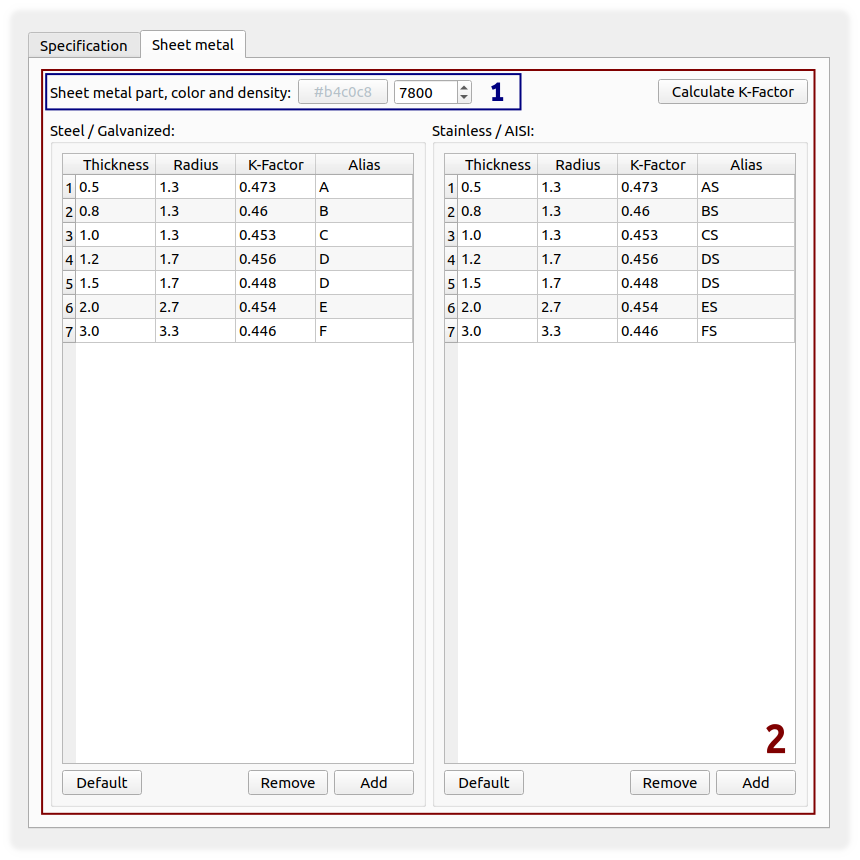
\includegraphics[width=1\textwidth]{img/pref_sm.png}
	\caption{Sheet metal preferences}
	\label{sec:pref_sm}
\end{figure}

\subsection{Area 4 -- Color for sheet metal part}
Color display for the object in HEX format, default value: \verb|#b4c0c8|.

\subsection{Area 5 -- Sheet steel parameters}
This table indicates the acceptable sheet metal \textbf{Thickness} for use and their parameters, such as the internal bending \textbf{Radius}, the \textbf{K-Factor} used when calculating the flat view (unfold).\\

\pagebreak

The \textbf{Calculate K-Factor} button automatically calculates the \textbf{k-factor} for each thickness using formulas from the strength of materials:

\begin{figure}[htp]
	\centering
	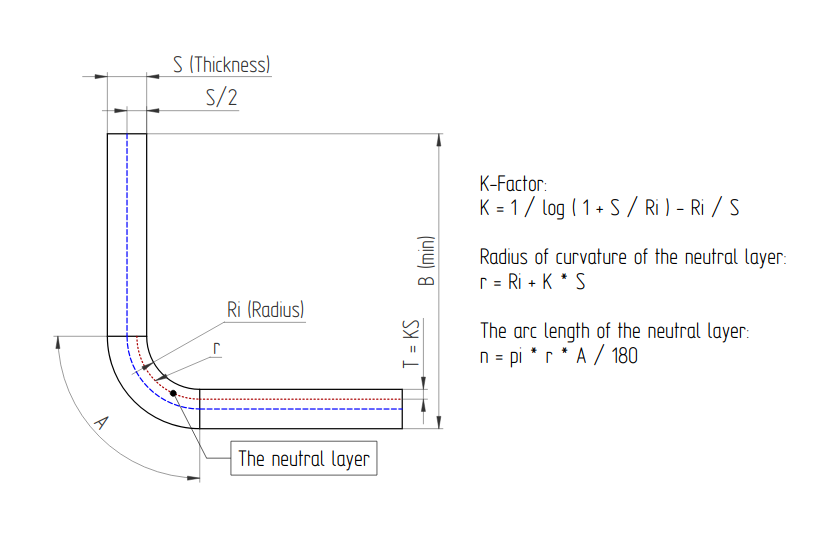
\includegraphics[width=1\textwidth]{img/k_en.png}
	\caption{Formulas for calculating sheet metal parameters}
	\label{sec:k}
\end{figure}

\pagebreak




\begin{figure}[htp]
	\centering
	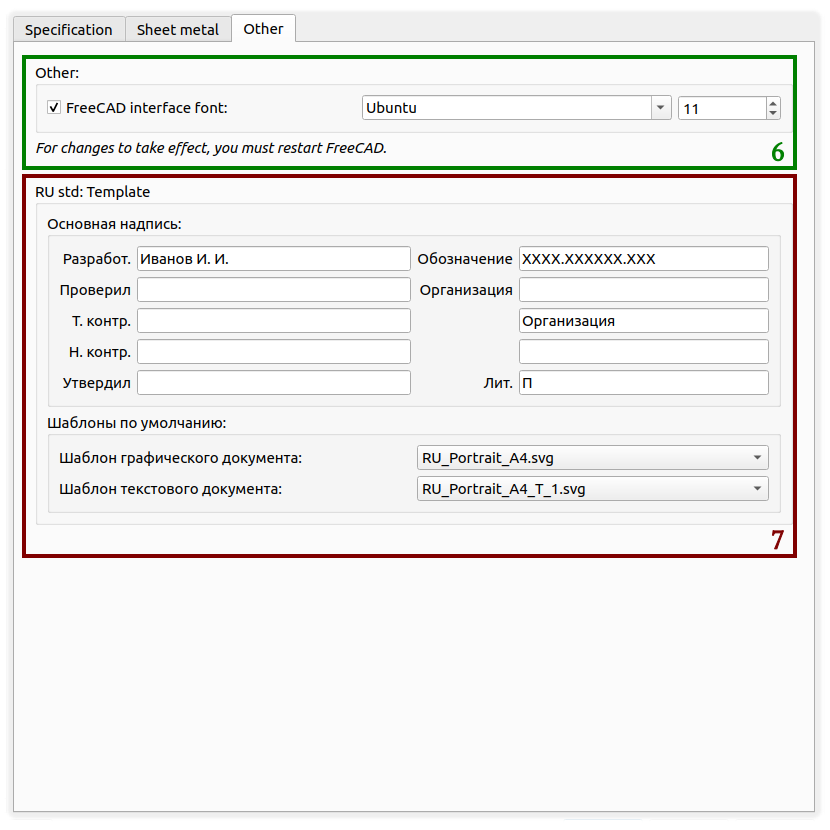
\includegraphics[width=1\textwidth]{img/pref_other.png}
	\caption{Additional preferences}
	\label{sec:pref_other}
\end{figure}

\subsection{Area 6 -- FreeCAD interface font options, additions}
In the \textbf{Font} area, you can specify the need to replace the standard program font and its parameters.\\The \textbf{Additions} area displays the presence of modules in the system that are necessary for the full operation of this workbench.

\subsection{Area 7 -- Parameters for Russian standard templates}
In this area you can specify values ​​for automatic filling of stamps when \hyperref[sec:6]{creating drawings} based on a template and automatic generation of a specification based on a model. The template specified in the corresponding field (шаблон текстового документа) will be selected as the first sheet of the specification.

\pagebreak




\begin{figure}[htp]
	\centering
	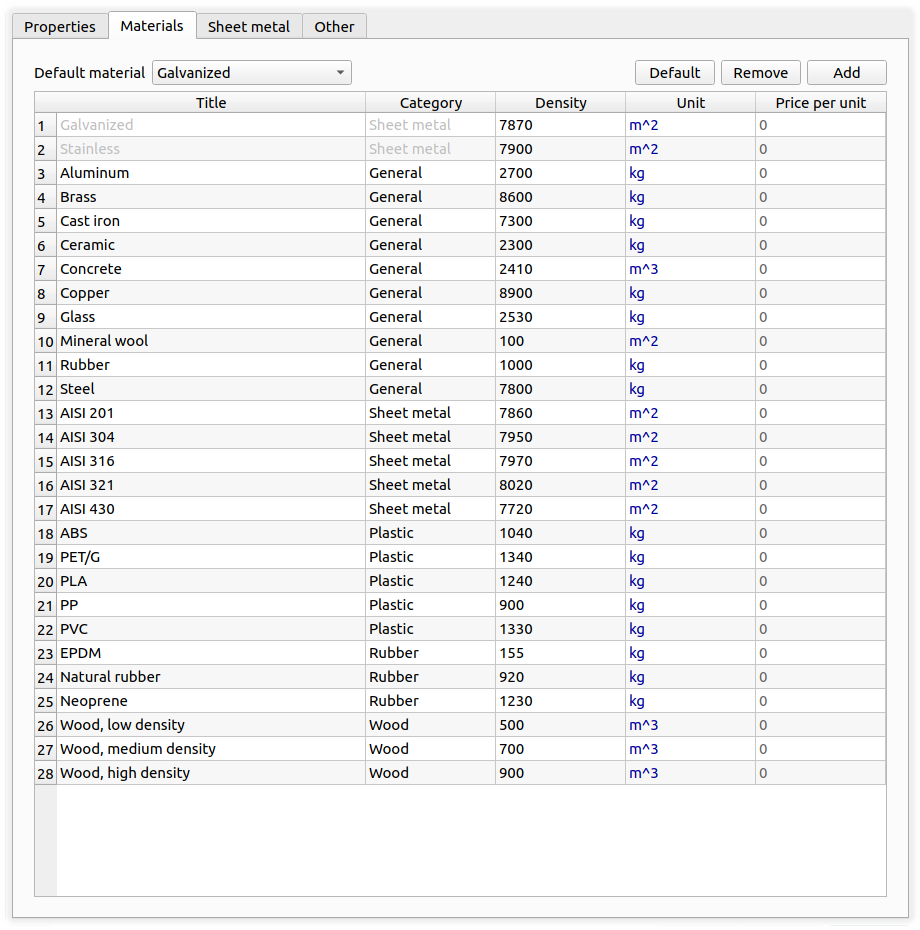
\includegraphics[width=1\textwidth]{img/pref_materials.png}
	\caption{Materials and their parameters}
	\label{sec:pref_materials}
\end{figure}

\subsection{Materials}
This tab contains a list of materials available for use. Parameters:
\begin{itemize}
    \item \textbf{Title} and \textbf{Category} -- name of the material and its category. For work with sheet metal parts, the choice of material is limited to the corresponding category.
    \item \textbf{Density} -- material density, can be used to automatically calculate the mass of an object, the «Weight» property.
    \item \textbf{Unit} and \textbf{Price per unit} -- price per unit of material, if necessary, can be used to calculate the cost of the element, the «Price» property.
\end{itemize}

\pagebreak




\section{Filling an object with properties}

To add properties, you need to select one or more objects and use the \hyperref[sec:5]{Add Properties} command on the toolbar.

\begin{figure}[htp]
	\centering
	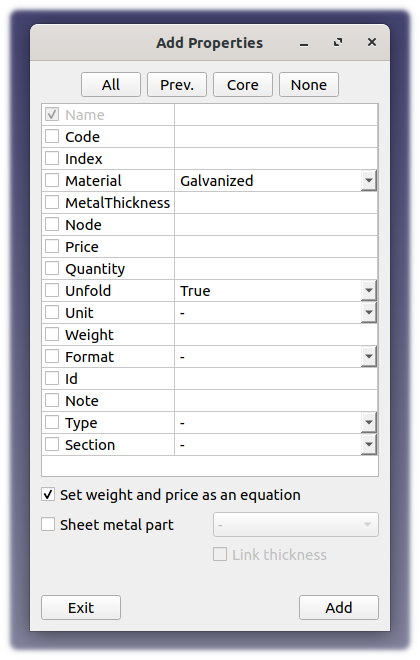
\includegraphics[scale=0.75]{img/properties_add.png}
	\caption{Interface \textbf{Add Properties}}
	\label{sec:properties_add}
\end{figure}

The entire list of available custom properties is visible in the command interface. You need to mark the ones you need and click \textbf{Add}.\\

Buttons \textbf{All}, \textbf{Core}, \textbf{None} -- select all properties, only the main ones and clear the selection.\\The \textbf{Prev.} button will highlight the properties added the last time the command was used.\\

Checkbox \textbf{Set weight and price as an equation} -- if enabled, the added properties «Weight» and «Price» will contain equations for automatic calculation of the corresponding parameters.

The \textbf{Sheet metal part} checkbox will check all the necessary properties for a sheet metal part, allow you to select the type of material and, if desired, associate the «MetalThickness» property with the thickness parameters of the object. Additionally, the element will be assigned a weight and color based on the parameters specified in the settings.\\

Note: During the process of assigning a \textbf{Name} and \textbf{Index}, the program tries to guess the property values ​​based on the \textbf{Label} of the object.

To automatically fill these properties, the name template must match: \textbf{«Index. Name - Copy»} or \textbf{«Index - Name - Copy»}. If the template matches, the values ​​will be filled in correctly -- \hyperref[sec:properties]{example}.

\pagebreak




\section{Bill of materials -- BOM}

To generate and work with BOM, you must use the \hyperref[sec:4]{Specification} command on the toolbar. Based on user properties, the program will generate a specification for any model (assembly), consider an example from the workbench:

\begin{figure}[htp]
	\centering
	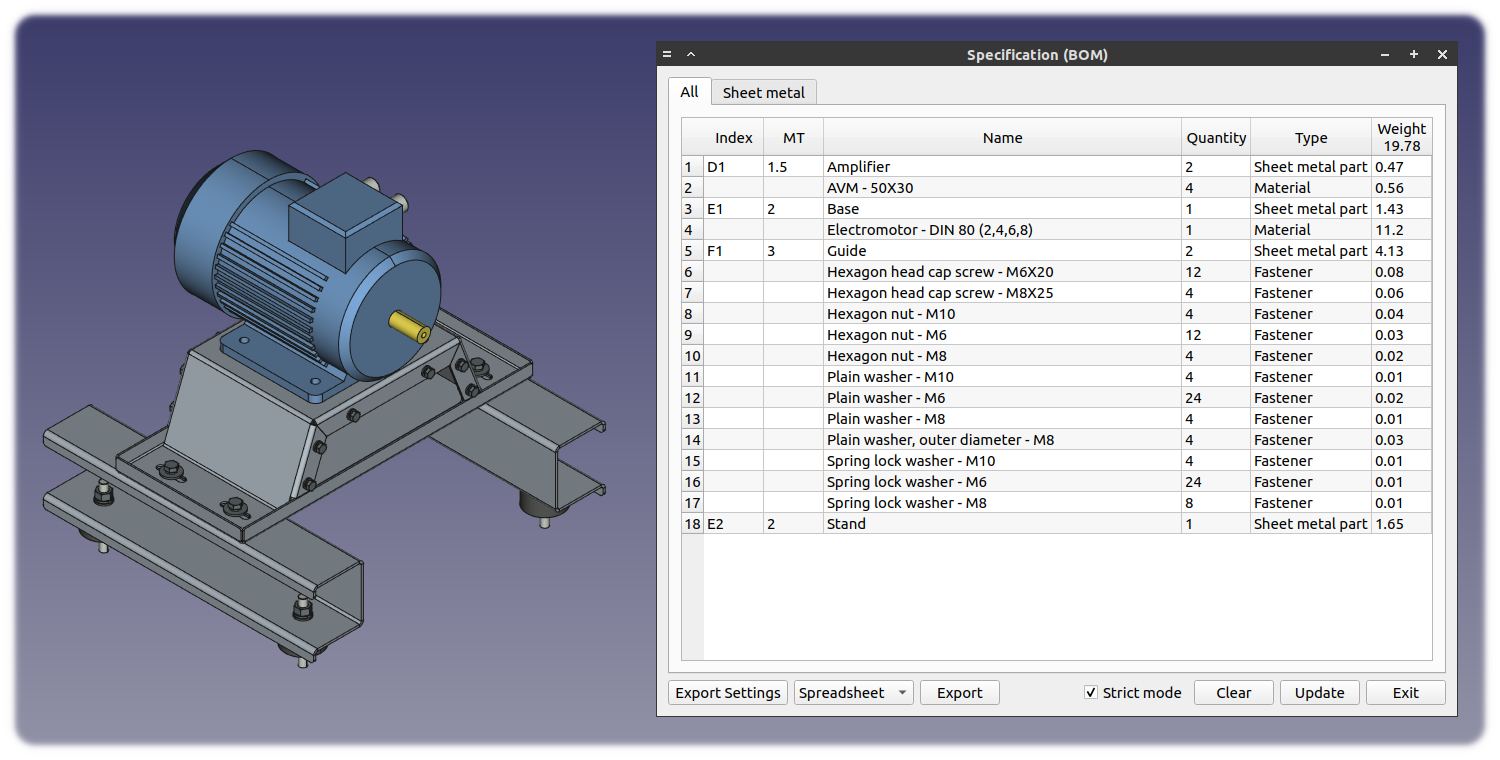
\includegraphics[width=1\textwidth]{img/specification_all.png}
	\caption{Bill of materials}
	\label{sec:specification_all}
\end{figure}

\begin{figure}[htp]
	\centering
	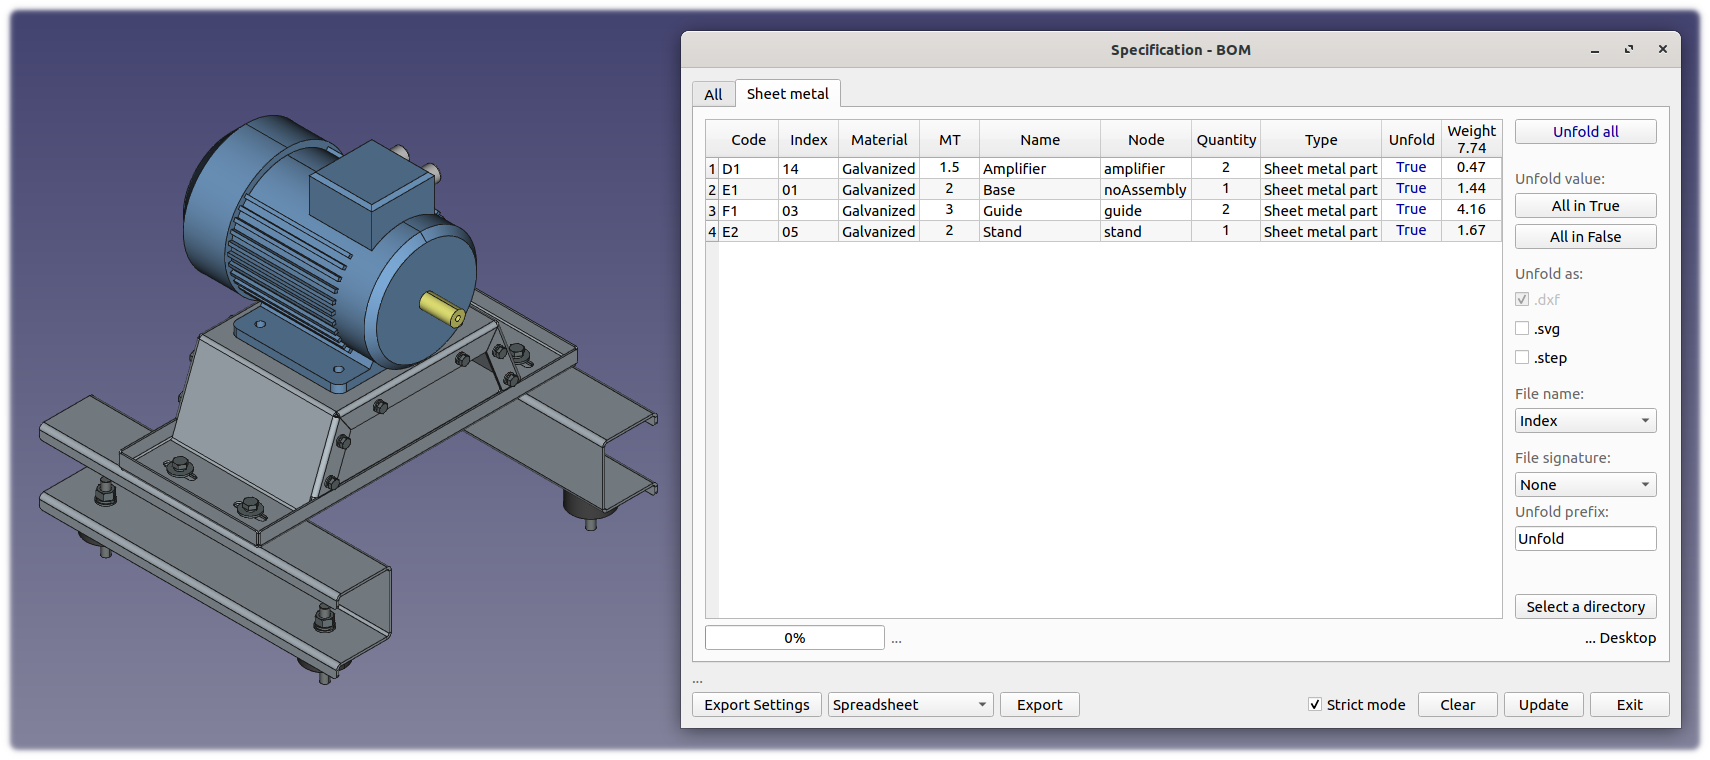
\includegraphics[width=1\textwidth]{img/specification_sm.png}
	\caption{Bill of materials, sheet metal parts}
	\label{sec:specification_sm}
\end{figure}

The specification interface contains two tabs:
\begin{itemize}
	\item \textbf{All} -- all objects.
	\item \textbf{Sheet metal} -- sheet metal objects.\\
\end{itemize}

\pagebreak

The \textbf{Strict mode} option -- if the checkbox is unchecked, the program will process all user\\ properties in your group -- \hyperref[sec:pref_specification]{figure 4: area 1}, not only those specified in the table (area 2).\\

There are two buttons on the \hyperref[sec:specification_sm]{all} specification tab:
\begin{itemize}
	\item \textbf{Indexing elements} -- Automatic indexing of positions for all elements\\included in the specification.
	\item \textbf{Update enumerations} -- update in model objects properties containing\\lists of predefined values. Useful after adding new values ​​to preferences.
	\item \textbf{Update equations} -- updating in model objects properties containing material-related equations, properties «Weight» and «Price».\\
\end{itemize}

Next we will look at \textbf{Sheet metal} objects -- this tab contains functions for their batch processing. The manufacturing process for such parts will in most cases require two elements:
\begin{itemize}
	\item \textbf{Blank (unfold)} -- a flat view of an object for nesting and processing on machines.
	\item \textbf{Part in 3D format (step)} -- for bending sheet metal.\\
\end{itemize}

All parts from the list generated based on the model (assembly), depending on the value of the \textbf{Unfold} property, can be processed and exported to external files, such as dxf, svg (unfolding) and step (3D).\\

\textbf{Select a directory} -- to save work results (the default value is the user's desktop).\\

\textbf{Unfold prefix} -- the name of the directory in which the files will be saved, as well as an option for signing the part.\\

\textbf{File signature} -- list of options for part signature. The signature is text in the file, inside the outline of the part, which can be useful when nesting. At the moment the function is only available for dxf format. When set to \textbf{None}, the signature is disabled. Important: This function requires the Python module: \href{https://pypi.org/project/ezdxf}{ezdxf}.\\

\textbf{File Name} -- the template by which the files will be named, for example,\\for the part \textbf{«E2 - Stand»} (\hyperref[sec:properties]{figure 5}) the names will be as follows:
\begin{itemize}
	\item \textbf{Name} = Stand (1).dxf
	\item \textbf{Code} = E2 (1).dxf
	\item \textbf{Index} = 05 (1).dxf
	\item \textbf{Code + Name} = (E2) Stand (1).dxf
	\item \textbf{Index + Name} = (05) Stand (1).dxf
\end{itemize}

The number in brackets at the end of the name is the copy number, if there are two or more identical parts in the assembly, they will be saved in separate files.\\

\pagebreak

After selecting the desired options and parameters, you can click the \textbf{Unfold} button and the program will save all received data in the specified path. The work process can be observed in the progress indicator and in FreeCAD, in the report panel (report view).\\

Important: The part files will be placed in additional directories, the names of which correspond to the name of the material and the thickness of the steel.




\section{Export specification}

The program can export a model (assembly) specification for subsequent viewing, editing or other use, available formats:
\begin{itemize}
	\item \href{https://wiki.freecad.org/Spreadsheet_Workbench}{\textbf{Spreadsheet}} -- FreeCAD spreadsheet workbench.
	\item \href{https://ru.wikipedia.org/wiki/JSON}{\textbf{json}} -- the most suitable option for subsequent automation.
	\item \href{https://en.wikipedia.org/wiki/Comma-separated_values}{\textbf{csv}} -- comma-separated values.
	\item \textbf{RU std} -- Unified System for Design Documentation, USDD -- Russia.
\end{itemize}

\begin{flushleft}First, let's look at the export options, button \textbf{Export Settings}.\end{flushleft}

\begin{figure}[htp]
	\centering
	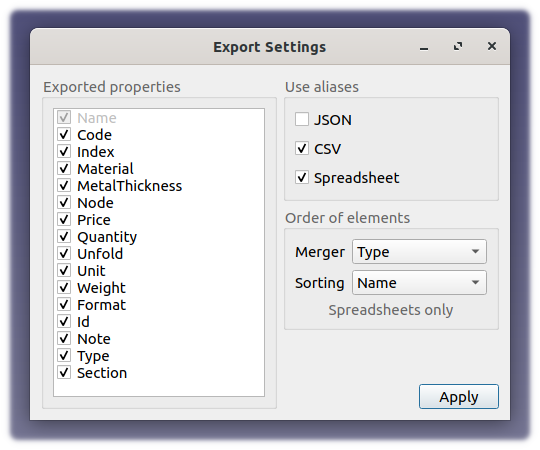
\includegraphics[scale=1]{img/specification_export.png}
	\caption{Specification export options}
	\label{sec:specification_export}
\end{figure}

On the left side of the interface you need to select the properties that will be available for export.\\

In the \textbf{Use aliases} area, you need to mark the formats in which aliases will be used, as a replacement for the \textbf{Title} property.\\

In the \textbf{Order of elements} area, you need to specify properties for grouping and sorting objects:
\begin{itemize}
	\item \textbf{Merger} -- a property by the value of which the elements will be grouped, the most suitable is the object \textbf{Type}, for example, display first all fasteners, then materials, then sheet metal parts.
	\item \textbf{Sorting} -- a property by the value of which objects will be sorted within a \textbf{Merger}, the most logical thing is to sort by \textbf{Index} or \textbf{Name}.
\end{itemize}

\pagebreak

Select the necessary options, the appropriate format and click the button \textbf{Export}.

\begin{figure}[htp]
	\centering
	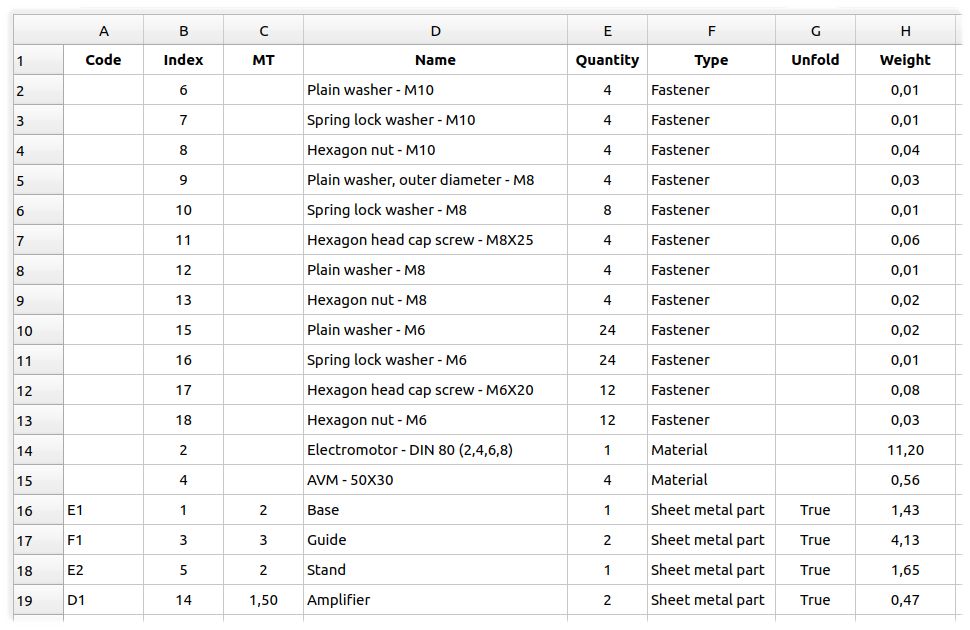
\includegraphics[width=1\textwidth]{img/specification_result.png}
	\caption{BOM export result}
	\label{sec:specification_result}
\end{figure}

\pagebreak




\section{Managing a parametric model}

The \hyperref[sec:3]{Model Control} command is available on the taskbar, the purpose of which is to launch a control program for a \textbf{parametric} model.\\

In my work, I was convinced that not one of the existing (for FreeCAD) assembly systems in combination with tables and equations is capable of providing such capabilities that are available from program code.

I write control files and interfaces for my parametric models, which are convenient to call with one command. To do this, next to the main model (assembly) file there should be two files named similarly to the main one.\\

In the samples supplied with the workbench, a simple example of a parametric model is available for study -- \verb|addFC/repo/example|

\begin{figure}[htp]
	\centering
	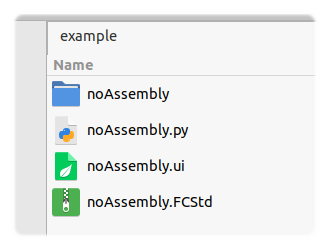
\includegraphics[scale=1]{img/example.png}
	\caption{Parametric model files}
	\label{sec:example}
\end{figure}

\begin{itemize}
	\item \textbf{.FCStd} -- main model file -- assembly.
	\item \textbf{.ui} -- user interface -- Qt.
	\item \textbf{.py} -- source code -- Python.
	\item \textbf{noAssembly} -- directory with additional files.
\end{itemize}

\pagebreak

Having opened the main file, you can call its control program using the \hyperref[sec:3]{Model Control} command:

\begin{figure}[htp]
	\centering
	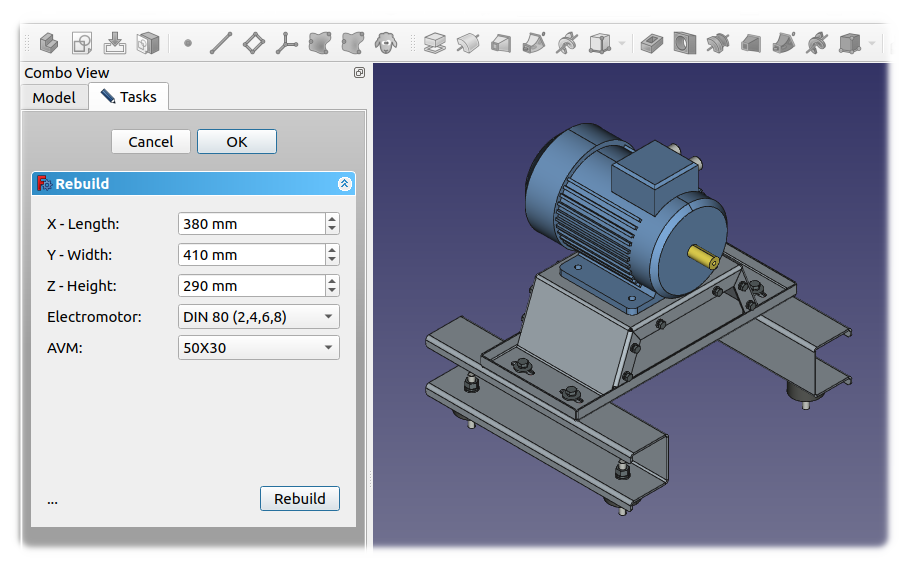
\includegraphics[width=1\textwidth]{img/example_mc.png}
	\caption{Parametric model management interface}
	\label{sec:example_mc}
\end{figure}

For convenience, the graphical user interface is built into the FreeCAD sidebar; after setting the necessary parameters and selecting components from the lists, click the \textbf{Rebuild} button -- the model will be updated.

\pagebreak




\section{Creating a pipeline using coordinates}

The \hyperref[sec:9]{Pipe} command allows you to create a pipeline using specified coordinates, \emph{the source of\\coordinates must be points} - either \textbf{Point} (Draft) or \textbf{Datum Point} (PartDesign). The first option is preferable.

Create and place points in 3D space, for convenience, they can be combined into a group, as shown in the example (figure 17).

Select the group with dots or any other parent element (in the example, pipe and path) in the project tree and click \hyperref[sec:9]{Pipe} on the toolbar.

\begin{figure}[htp]
	\centering
	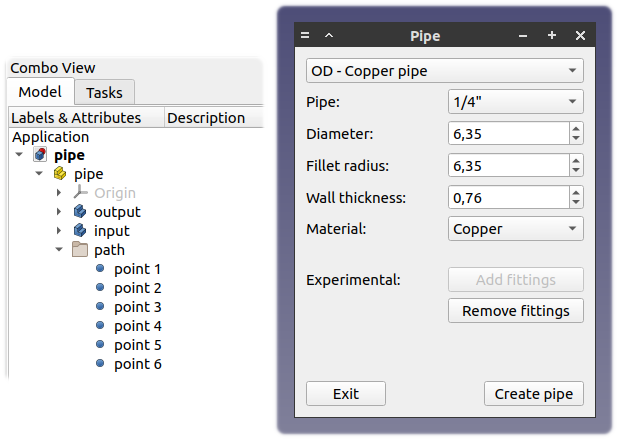
\includegraphics[scale=1]{img/pipe.png}
	\caption{Coordinate points and interface \textbf{Pipe}}
	\label{sec:pipe}
\end{figure}

The interface provides:
\begin{itemize}
	\item \textbf{Top drop down list} -- these are pipe templates, available options:
	\begin{itemize}
		\item \textbf{OD - Copper pipe} -- inch copper pipes, range from 1/4" to 4+1/8".
		\item \textbf{DN - Nominal pipe size} -- NPS.
		\item \textbf{DN - ВГП (водогазопроводная)} -- GOST 3262-75 (Russia).
	\end{itemize}
	\item \textbf{Pipe} -- pipe size option from selected template.
	\item \textbf{Diameter} -- diameter, OD -- external, DN -- nominal bore.
	\item \textbf{Fillet radius} -- pipe bending radius.
	\item \textbf{Wall thickness} -- pipe wall thickness.
	\item \textbf{Material} -- pipe material, color and density values.
\end{itemize}

If necessary, the values ​​of diameter, bend and wall thickness can be specified manually by changing the values ​​of the corresponding fields.\\

After selecting the required parameters, click \textbf{Create pipe}.

\begin{figure}[htp]
	\centering
	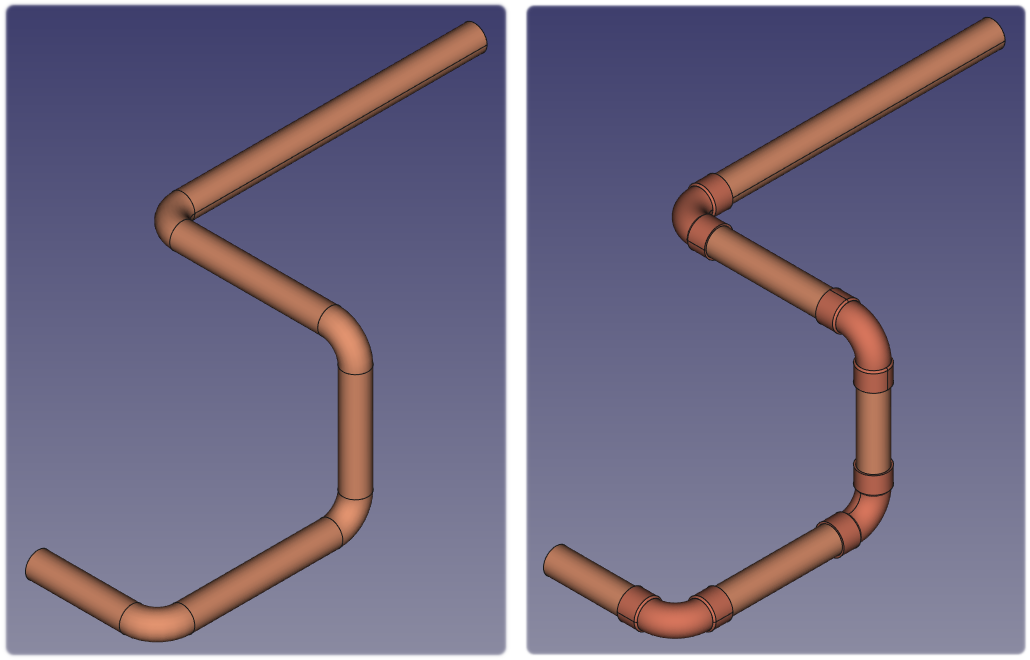
\includegraphics[width=1\textwidth]{img/pipe_result.png}
	\caption{The result of the \textbf{Pipe} operation}
	\label{sec:pipe_result}
\end{figure}

The program will receive the coordinates of all points (the points themselves will be sorted by \textbf{Label}, in ascending order) and will build a pipeline with the previously specified parameters.

The image shows the result of the team's work, on the right is an option with added fittings,\\command \textbf{And fittings}.

\pagebreak




\section{Exploded view}

The \hyperref[sec:8]{Explode} command is responsible for creating an exploded view -- a sketch view of a design (assembly) with its component parts exploded, which allows you to convey information about the product in a simpler and easier to understand form. The tool allows you to create, animate and save views.

\begin{figure}[htp]
	\centering
	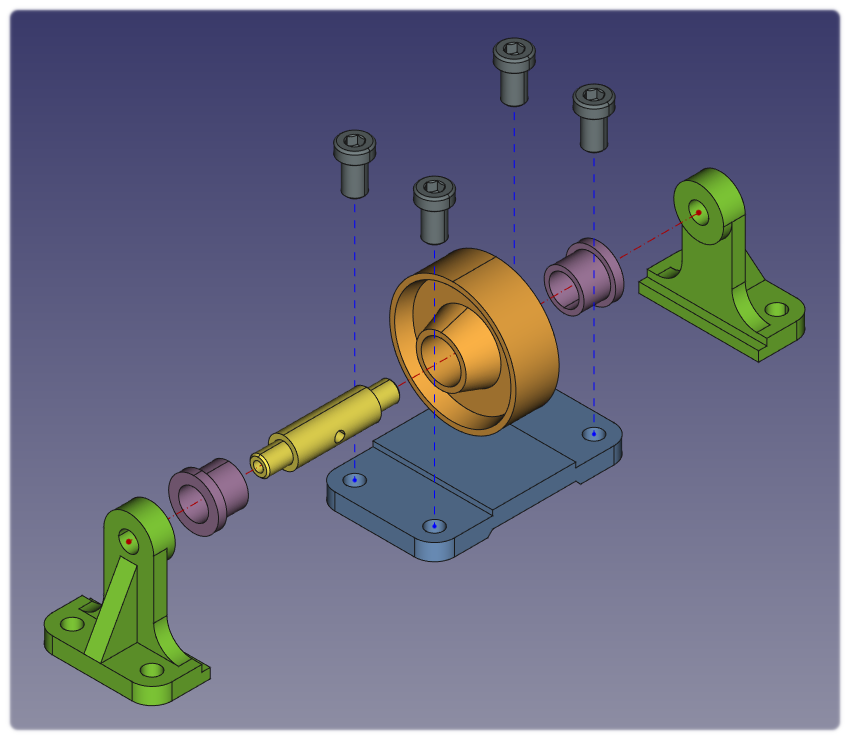
\includegraphics[scale=0.42]{img/exploded_m_result.png}
	\caption{\textbf{Explode}: exploded view of model}
	\label{sec:exploded_m_result}
\end{figure}

\begin{figure}[htp]
	\centering
	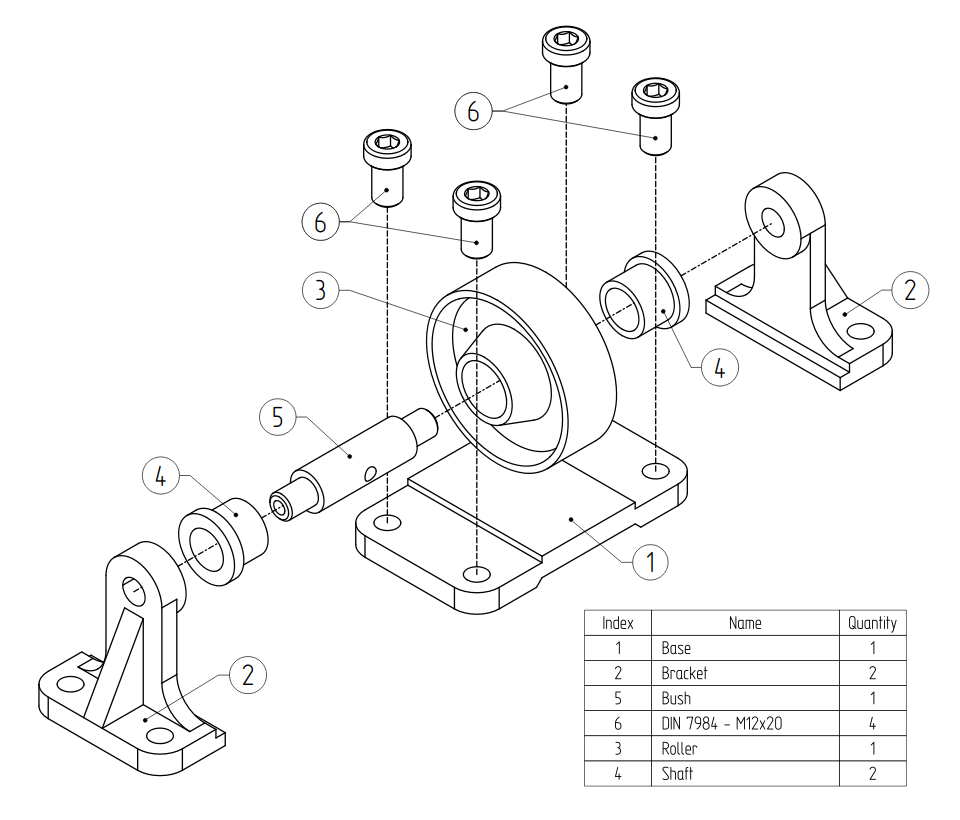
\includegraphics[scale=0.42]{img/exploded_d_result.png}
	\caption{\textbf{Explode}: export exploded view to drawing}
	\label{sec:exploded_d_result}
\end{figure}

\pagebreak

\begin{figure}[htp]
	\centering
	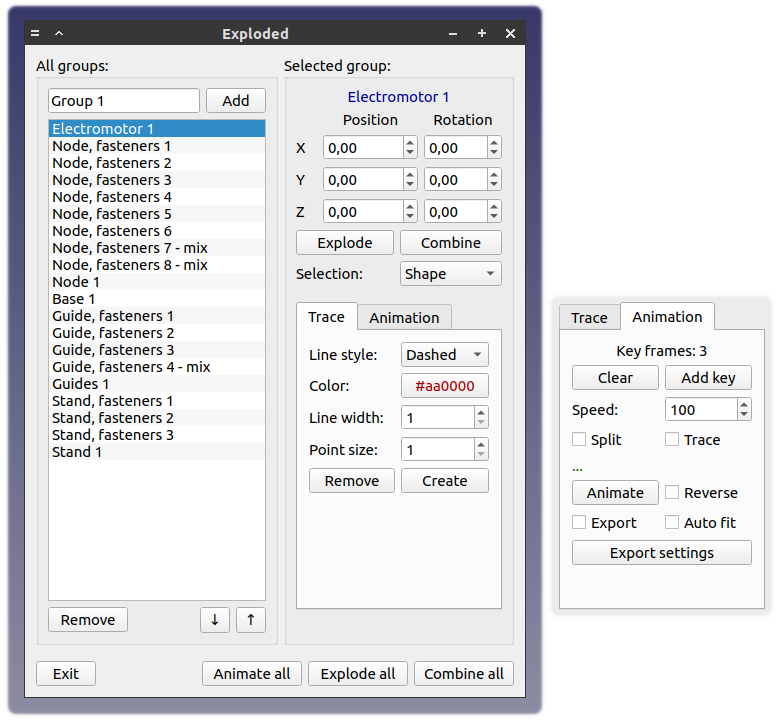
\includegraphics[width=1\textwidth]{img/exploded.png}
	\caption{\textbf{Explode} interface}
	\label{sec:exploded}
\end{figure}

On the left side of the interface there are groups, a group is one or more combined elements. To create a group, you need to select objects in the project tree or 3D view window and click the \textbf{Add} button. Created groups can be \textbf{Remove} and moved by positions (arrows: up, down).

Double clicking on the group name will make it active, area: \textbf{Selected group}.

Elements of the active group can be moved by coordinates (\textbf{Position}) and rotated by axes\\(\textbf{Rotation}). All actions are displayed in the 3D view window and are automatically saved.

The \textbf{Combine} button returns all elements in the group to their original positions.

The \textbf{Explode} button moves the group objects to the location specified by the user.\\

Список \textbf{Selection} - appearance of selected objects:
\begin{itemize}
	\item \textbf{Shape} -- fill an object with color (standard selection).
	\item \textbf{BoundBox} -- frame around object.
	\item \textbf{None} -- no selection.
\end{itemize}

\pagebreak




The \textbf{Trace} tab is responsible for guides - these are visual lines from the original position of the element to its current location specified by the user.
\begin{itemize}
	\item \textbf{Line style}, \textbf{Color} -- the style of the guide line and its color.
	\item \textbf{Line width}, \textbf{Point size} -- line thickness and size of start and end points.
	\item \textbf{Create}, \textbf{Remove} -- create and delete guide lines for a group.
\end{itemize}
An example of guides can be seen in images \hyperref[sec:exploded_m_result]{19} and \hyperref[sec:exploded_d_result]{20}.\\

The \textbf{Animation} tab is responsible for animating the exploded view and exporting the animation to a video file. The general principle of operation is as follows: after moving and/or rotating an object, you can \textbf{Add key} frame, the program animates the movement and/or rotation of objects from the initial location to the position specified by the key frame. The number of frames is unlimited. The current number of frames is displayed in the field: \textbf{Key frames}. The \textbf{Clear} button will delete all created key frames for the group.\\

\textbf{Speed} -- the animation playback speed for the current keyframe..

\textbf{Split} -- if checked, the objects in the group will be animated sequentially.

\textbf{Trace} -- display guide lines for objects during animation.\\

\textbf{Animate} button -- play animation by keyframes.

\textbf{Reverse} checkbox, if checked -- the animation will be played in reverse.

\textbf{Auto fit} -- automatic camera positioning to display all elements.

\textbf{Export} -- when playing, save the animation to a video file.\\

Important: for full functionality you need:
\begin{itemize}
	\item Python \href{https://pypi.org/project/numpy}{NumPy} module for animation.
	\item \href{https://www.ffmpeg.org}{FFmpeg} library for exporting animation to a video file.
\end{itemize}

\pagebreak




\begin{figure}[htp]
	\centering
	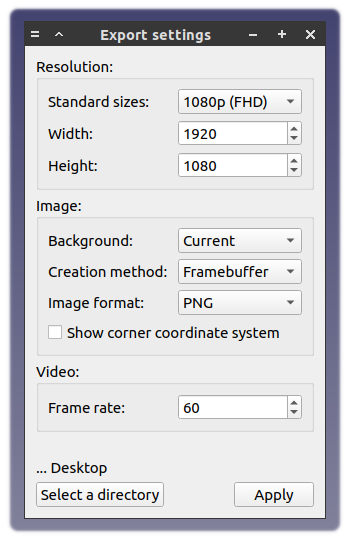
\includegraphics[scale=1]{img/exploded_es.png}
	\caption{Export settings}
	\label{sec:exploded_es}
\end{figure}

Export options are the video file \textbf{Resolution}, \textbf{Frame rate}, directory for saving the result -- the \textbf{Select a directory} button, and also some frame-by-frame image settings:

\begin{itemize}
	\item \textbf{Image format} -- PNG (higher quality) and JPG (faster).
	\item \href{https://wiki.freecad.org/Std_ViewScreenShot}{\textbf{Background} and \textbf{Creation method.}}
\end{itemize}




\section{Библиотека элементов и узлов}

Coming soon...




\end{document}